%% Manuscript for Artificial Intelligence Review (Springer Nature), journal 10462.
%% Springer Nature LaTeX template (December 2024), Basic Springer Nature reference style,
%% author-year citations. Compile: pdflatex, bibtex, pdflatex, pdflatex.
%% All files sit in one folder as the journal requires (no subfolders).
\documentclass[pdflatex,sn-basic]{sn-jnl}

\usepackage{graphicx}%
\usepackage{multirow}%
\usepackage{amsmath,amssymb,amsfonts}%
\usepackage{xcolor}%
\usepackage{textcomp}%
\usepackage{manyfoot}%
\usepackage{booktabs}%
\usepackage{array}%
\usepackage{tabularx}%
\usepackage{longtable}%

\newcolumntype{L}{>{\raggedright\arraybackslash}X}
\newcolumntype{P}[1]{>{\raggedright\arraybackslash}p{#1}}
\providecommand{\doi}[1]{\url{https://doi.org/#1}}
%% Items the author still has to supply or confirm (see open_questions.md).
\newcommand{\tbc}[1]{\textbf{[#1]}}
\setlength{\LTcapwidth}{\textwidth}

\raggedbottom

\begin{document}

\title[Reinforcement learning in IT incident triage: a systematic review]{Reinforcement Learning for Investigating, Acting and Escalating in IT Incident Triage and Response: A Systematic Literature Review}

\author*{\fnm{Charis} \sur{Opol}}\email{B29654@students.ucu.ac.ug}\email{charisopol@gmail.com}

\affil*{\orgdiv{Department of Computing and Technology, Faculty of Engineering, Design and Technology}, \orgname{Uganda Christian University}, \orgaddress{\city{\tbc{city}}, \state{\tbc{state or region, if used}}, \country{Uganda}}}

\abstract{Information technology (IT) support teams must decide how to handle an incident before its cause is known: investigate further, apply a fix, or pass the incident to a person. This review examines how reinforcement learning and related sequential methods are applied to IT incident handling, which of these three decisions their agents make, how operational rules are enforced, and how the agents are evaluated. Following the Preferred Reporting Items for Systematic Reviews and Meta-Analyses (PRISMA) 2020 guideline, searches of Scopus, IEEE Xplore and the ACM Digital Library on 23 October 2026 returned 4,399 records. After 73 duplicates were removed and 4,195 records were filtered out automatically, 131 were screened, 40 reports were assessed in full, and 34 studies (2020--2026) were included and appraised with an eight-item checklist. Four studies represent the hidden incident state with an explicit belief. Seventeen give the agent an information-gathering action and 7 include escalation to a person; only one combines all three decisions, and its escalation is fixed by design rather than learned. Five use a hard filter or shield, and 3 report what happens to a blocked or uncertain decision. Decision quality is measured in 31 studies, escalation behaviour in 5, constraint compliance in 4, and robustness in 15. The evidence is recent (27 studies from 2025 or 2026) and of uneven quality: 12 meet at most two checklist items. No study reports a single policy that learns to investigate, act or escalate for IT service incidents under explicit rules.}

\keywords{Reinforcement learning, IT incident management, Incident triage, Escalation, Safe reinforcement learning, Systematic literature review}

\maketitle

\noindent ORCID: Charis Opol \url{https://orcid.org/0009-0003-7417-7984}

\bmhead{Acknowledgements}
\tbc{Acknowledgements to be supplied by the author, or this section deleted. The names of any funding organisations must be written in full.}

\section{Introduction}\label{sec:intro}

Organisations depend on information technology (IT) services that are expected to remain available, and incident management is the process that restores those services when they fail. \citet{chen2020} describe it as the process of detecting a service problem, creating an incident, determining its cause, restoring the service, and capturing knowledge to prevent a recurrence. Triage is the stage at which a reported incident is assessed and directed towards resolution. \citet{chen2020} define it as engaging the team responsible for investigating the problem, and \citet{remil2024} use the term more broadly for the prioritisation, assignment and classification of incidents. In both descriptions, triage is a set of decisions made before the cause of the incident is known. The abbreviations used in this review are listed in Table~\ref{tab:abbrev}.

\begin{table}[!htbp]
\caption{Abbreviations used in this review and their meanings}\label{tab:abbrev}
\footnotesize
\begin{tabularx}{\textwidth}{@{}lL@{}}
\toprule
Abbreviation & Meaning \\
\midrule
AIOps & Artificial Intelligence for IT Operations \\
CAGE & Cyber Autonomy Gym for Experimentation \\
CMDP & Constrained Markov Decision Process \\
DQN & Deep Q-Network \\
EC / IC & Exclusion criterion / Inclusion criterion \\
ICS & Industrial Control System \\
IDS & Intrusion detection system \\
IoT & Internet of Things \\
IT & Information technology \\
LLM & Large Language Model \\
MCC & Matthews Correlation Coefficient \\
MDP & Markov Decision Process \\
MTTR & Mean Time to Recovery or Resolution \\
OT & Operational technology \\
POMDP & Partially Observable Markov Decision Process \\
PPO & Proximal Policy Optimisation \\
PRISMA & Preferred Reporting Items for Systematic Reviews and Meta-Analyses \\
RCA & Root Cause Analysis \\
RL & Reinforcement Learning \\
ROC-AUC & Area under the receiver operating characteristic curve \\
SO / SRQ & Specific Objective / Systematic Review Question \\
SOC & Security Operations Centre \\
\botrule
\end{tabularx}
\end{table}

These decisions are difficult because the evidence available when they are made is often incomplete or conflicting. In their study of incident management at Microsoft, \citet{chen2020} found that distinct problems can produce similar symptoms, so that the symptoms alone may not identify the responsible team. \citet{remil2024} note that data in real IT environments is commonly noisy and incomplete. Yet many triage models produce one prediction per incident report and are evaluated with classification or ranking metrics \citep{remil2024}. A model of this kind returns an answer for every report. It has no way to state that more evidence is needed first, and no way to pass the incident to a person.

Reinforcement learning (RL) offers a different framing. In RL, an agent learns a policy, which is a rule for choosing actions, by acting in an environment and receiving rewards that reflect the consequences of its actions \citep{sutton2018}. When the agent cannot observe the true state of the environment, the problem can be described as a partially observable Markov decision process (POMDP), in which the agent keeps a belief about the hidden state and may choose an action for the information it yields, weighing the cost of that information against its value \citep{kaelbling1998}. Under this framing, triage becomes a sequence of decisions: the agent can gather more evidence, recommend an action, or hand the incident to a human expert.

Two further requirements follow when such an agent is meant for IT operations. The first is that its actions must respect operational rules. A reward signal alone does not ensure this, because penalising an undesirable action in the reward does not guarantee that the agent never selects it \citep{konighofer2025}, and \citet{remil2024} state that automatic healing actions need to be executed safely. The second is that the agent must know when to involve a person. Learning to defer trains a model to decide when a human should take over \citep{madras2018}, and recent work treats escalation as a decision with costs in both directions, since a reviewer's attention is limited \citep{turan2026}.

The literature review for the project of which this review is part (Chapter Two of the project report) found that these strands have developed largely apart. Studies of information gathering let an agent choose between looking further and deciding \citep{janisch2019,kim2025}, studies of deferral let it choose between deciding and handing over \citep{madras2018,joshi2023}, and a shielded agent proposed for incident response selects responses without choosing whether to investigate or escalate \citep{alauthman2026}. That review was thematic and not systematic. It drew on a core set of collected publications and on a database search run on 13 October 2026, which returned 10,694 records that were filtered by keyword and not screened. Its conclusions about gaps were therefore conclusions about the literature it had read. This review replaces that search with a narrower, documented one, screens its results against fixed criteria, and synthesises what the included studies report.

The project plans an RL agent for IT incident triage that chooses among requesting a diagnostic check, recommending a fix that the organisation's operational rules permit, and escalating to a human expert, with every proposal checked by an independent rule-based mechanism. The agent is to be trained and evaluated in simulation. Because this review prepares for that study, it could lean towards the planned design. Three measures limit this. The eligibility criteria were written before screening, the decisions that required interpretation are stated in Section~\ref{sec:screening}, and the outcome of every report sought is listed in Table~S1 of Online Resource~1. These measures do not remove the risk, because the screening and extraction were not independently duplicated (Section~\ref{sec:limitations}).

The review addresses five systematic review questions (SRQ1--SRQ5):
\begin{itemize}
\item \textbf{SRQ1:} How have IT incident handling tasks been formulated as Markov decision process (MDP), POMDP or RL problems, and how is incomplete or conflicting evidence represented in them?
\item \textbf{SRQ2:} Which decisions do the agents make (gathering information, recommending or taking an action, escalating to a human), and does any study combine all three?
\item \textbf{SRQ3:} How are operational constraints enforced, for example by a shield, action masking, constrained optimisation, a reward penalty or human approval, and what happens when an action is blocked?
\item \textbf{SRQ4:} Which environments, datasets, baselines and evaluation metrics are used?
\item \textbf{SRQ5:} How is robustness to missing, unreliable or ambiguous evidence evaluated, and what results are reported?
\end{itemize}

The general objective is to systematically identify and synthesise peer-reviewed studies that apply RL or sequential decision-making to IT incident management, with attention to how they represent uncertain evidence, which decisions the agent makes, how constraints are enforced, and how the agents are evaluated. Table~\ref{tab:objectives} gives the five specific objectives (SO1--SO5), the question each answers, the research question of the project that it informs, and the gap that motivated it. The gaps in the table are those stated by the project's thematic review before this search; Section~\ref{sec:discussion} returns to each of them in the light of the included evidence.

\begin{table}[!htbp]
\caption{Specific objectives of the review (SO1--SO5), the systematic review question (SRQ) that each answers, the research question (RQ1--RQ5) of the author's project that each informs, and the gap, as stated by the project's earlier thematic review, that motivated each objective}\label{tab:objectives}
\footnotesize
\begin{tabularx}{\textwidth}{@{}P{2.9cm}P{1.0cm}P{2.1cm}L@{}}
\toprule
Specific objective & Review question & Project question informed & Gap that motivated it (from the thematic review) \\
\midrule
SO1: Identify which incident tasks have been formulated as sequential decision problems, and how they represent uncertain evidence & SRQ1 & RQ1 (representation of ambiguous scenarios) & The environments used in the reviewed studies model cyberattacks and microservice faults, and none lets the ambiguity of IT service incidents be varied \citep{hammar2025,dunsin2025,wang2023hrlhf}. \\
SO2: Classify the decisions the agents make & SRQ2 & RQ2 (investigate, recommend, escalate) & Information gathering and deferral have been studied separately; no reviewed study trained one policy to choose among all three options for IT incident triage \citep{janisch2019,kim2025,madras2018,joshi2023}. \\
SO3: Analyse how constraints are enforced and what is reported about blocked actions & SRQ3 & RQ3 (rule-based safety mechanism) & Shields have been demonstrated mainly on control tasks, and the reviewed literature did not report how a rule mechanism behaves when the agent can also investigate or escalate \citep{alshiekh2018,konighofer2025,alauthman2026}. \\
SO4: Catalogue environments, datasets, baselines and metrics & SRQ4 & RQ4 (comparison with baselines) & Decision quality, investigation cost, escalation and constraint compliance had each been measured, but not together for one agent \citep{remil2024,levy2026,pacella2026}. \\
SO5: Synthesise how robustness to increasing ambiguity is tested & SRQ5 & RQ5 (robustness) & Robustness had been tested for decision accuracy and for the validity of shields, but not for the mix of investigating, recommending and escalating \citep{kim2025,hammar2025,hamel2026}. \\
\botrule
\end{tabularx}
\end{table}

\section{Methods}
\label{sec:method}

This study is a systematic literature review reported according to the Preferred Reporting Items for Systematic Reviews and Meta-Analyses (PRISMA) 2020 guideline \citep{page2021} and guided by the review procedure for computing proposed by \citet{kitchenham2007}. A systematic approach was chosen because it makes the search, selection and extraction of studies transparent and reproducible, and because the earlier search for the project returned too many records to screen. The design follows the five objectives and questions in Table~\ref{tab:objectives}. The protocol was not registered. Every count reported below is generated from the screening and extraction records that accompany this review (Section~\ref{sec:records}).

\subsection{Information Sources}

Three databases were searched: Scopus, IEEE Xplore and the ACM Digital Library. Scopus was the primary source for its broad indexing. IEEE Xplore was chosen for its coverage of network, service management and security venues, and the ACM Digital Library for software engineering and systems venues, where much work on artificial intelligence for IT operations (AIOps) appears. The searches were run on 23 October 2026. The Scopus and ACM Digital Library searches used the all-fields option of each site. The IEEE Xplore search was limited to open-access records.

Other sources were considered and not used. SpringerLink and SIAM, which were searched for the project's earlier review, were dropped: the SpringerLink export of that search contained no abstracts, and SIAM returned three records. Web of Science was not searched. arXiv was not searched directly, so preprints could have entered only through citation searching, which was planned but not carried out (Section~\ref{sec:other}).

\subsection{Search Strategy}

The search was designed to be narrow. The earlier search had combined a block of terms for the learning approach, a block for uncertainty and oversight, and a block for the incident-management setting. Single words such as ``uncertainty'' and ``triage'' match large bodies of unrelated work, including medical triage and traffic incidents. The new string therefore anchors the review on the intersection of two concepts, the RL or sequential-decision method (block~A) and the IT incident setting (block~B), expressed as exact phrases, and adds a block of decision terms (block~C). Synonyms within a block were joined with OR and the blocks were joined with AND. Table~\ref{tab:keywords} lists the keywords and shows where each appears.

\begin{table}[!htbp]
\caption{Keywords used to build the search strings and the block of the string in which each appears (A, method; B, setting; C, decision)}\label{tab:keywords}
\footnotesize
\begin{tabularx}{\textwidth}{@{}lLL@{}}
\toprule
No. & Keyword & Block \\
\midrule
1 & Reinforcement learning & A (method) \\
2 & Sequential decision-making & A, as MDP, POMDP and bandit terms \\
3 & POMDP & A \\
4 & IT incident management & B (setting) \\
5 & Incident triage & B \\
6 & Incident response & B \\
7 & AIOps & B \\
8 & Root cause analysis & B, limited to computing systems \\
9 & Escalation & C (decision) \\
10 & Human-in-the-loop & C \\
11 & Information gathering & C \\
12 & Safe reinforcement learning & C \\
13 & Shielding & C \\
14 & Operational constraints & C \\
\botrule
\end{tabularx}
\end{table}

Table~\ref{tab:strings} gives the strings exactly as they were run. The Scopus and ACM Digital Library strings are identical. Both end with a fourth group of quoted years; because the searches ran over all fields, these terms match any record that mentions one of the years anywhere and do not restrict the publication year. The IEEE Xplore string differs in four respects: it uses the Scopus proximity operator \texttt{W/5} for the root-cause clause, it spells several terms in full instead of truncating them, it has no year terms, and it was limited to open access. Whether IEEE Xplore interpreted \texttt{W/5} as intended was not tested.

\begin{table}[!htbp]
\caption{Search strings exactly as run on 23 October 2026 in each database, and the number of records exported from each}\label{tab:strings}
\scriptsize
\begin{tabularx}{\textwidth}{@{}P{2.2cm}L@{}}
\toprule
Database & String as run \\
\midrule
Scopus (all fields) and ACM Digital Library (all fields) & \texttt{( "reinforcement learning" OR "deep Q-network*" OR "Q-learning" OR "policy gradient" OR "actor-critic" OR "proximal policy optimi*" OR "Markov decision process*" OR "partially observable Markov" OR POMDP OR "contextual bandit*" OR "multi-armed bandit*" ) AND ( "incident management" OR "incident response" OR "incident triage" OR "incident handling" OR "incident resolution" OR "incident mitigation" OR AIOps OR "IT operations" OR "IT service management" OR ITSM OR "site reliability" OR "service desk" OR "help desk" OR "trouble ticket*" OR "ticket routing" OR "ticket assignment" OR "alert triage" OR "alert prioriti*" OR "security operations cent*" OR "automated remediation" OR ( "root cause" AND ( microservice* OR cloud OR "online service*" OR "IT system*" ) ) ) AND ( triage OR escalat* OR defer* OR "human-in-the-loop" OR "human in the loop" OR "human oversight" OR investigat* OR diagnos* OR "information gathering" OR "information acquisition" OR remediat* OR mitigat* OR constrain* OR shield* OR "safe reinforcement learning" OR "action mask*" OR "partial* observ*" OR uncertain* OR ambigu* ) AND ( "2015" OR "2016" OR "2017" OR "2018" OR "2019" OR "2020" OR "2021" OR "2022" OR "2023" OR "2024" OR "2025" OR "2026" )} \\
\addlinespace
IEEE Xplore (open access only) & \texttt{( "reinforcement learning" OR "deep Q-network*" OR "Q-learning" OR "policy gradient" OR "actor-critic" OR "proximal policy optimization" OR "Markov decision process*" OR "partially observable Markov" OR POMDP OR "contextual bandit*" OR "multi-armed bandit*" ) AND ( "incident management" OR "incident response" OR "incident triage" OR "incident handling" OR "incident resolution" OR "incident mitigation" OR AIOps OR "IT operations" OR "IT service management" OR ITSM OR "site reliability" OR "service desk" OR "help desk" OR "trouble ticket*" OR "ticket routing" OR "ticket assignment" OR "alert triage" OR "alert prioritization" OR "security operations center" OR "automated remediation" OR ("root cause" W/5 (microservices OR cloud OR "online services" OR "IT systems")) ) AND ( triage OR escalation OR defer* OR "human-in-the-loop" OR "human in the loop" OR "human oversight" OR investigation OR diagnosis OR "information gathering" OR "information acquisition" OR remediation OR mitigation OR constraint* OR shield* OR "safe reinforcement learning" OR "action masking" OR "partial observability" OR uncertainty OR ambiguity )} \\
\midrule
Records exported & Scopus 3394; ACM Digital Library 1000; IEEE Xplore 5. Total: 4399. \\
\botrule
\end{tabularx}
\end{table}

The all-fields searches returned many records unrelated to the questions, because a record matched if the terms appeared anywhere, including in reference lists and front matter. Among the ACM records, 630 were whole proceedings volumes. The exports were therefore filtered again with a script, as described in Section~\ref{sec:records}, before any record was screened.

The string was checked against a benchmark set of seven studies already known to be relevant: \citet{alauthman2026}, \citet{hammar2025}, \citet{hammar2026belief}, \citet{wang2023hrlhf}, \citet{ding2023}, \citet{ren2025} and \citet{dunsin2025}. Six of the seven are among the exported records; Ren et al.\ is not. When block~C was re-applied to the titles, abstracts and keywords of the exports, it removed two of the six, the studies of Hammar and Li and of Hammar et al., whose abstracts use none of its terms. Block~C was therefore not re-applied in the automated filtering, and its terms were kept as data items in the extraction form (Section~\ref{sec:extraction}).

\subsection{Eligibility Criteria}

The inclusion criteria (IC1--IC5) and exclusion criteria (EC1--EC7) in Table~\ref{tab:criteria} were written before screening and are linked to the research questions. Studies from security operations and cybersecurity incident response were kept within scope, because much of the RL work on incident handling comes from that setting. Their setting was recorded during extraction so that it could be separated from IT service incidents in the synthesis.

\begin{table}[!htbp]
\caption{Eligibility criteria: the inclusion criteria (IC1--IC5) and exclusion criteria (EC1--EC7) for each aspect of a study, applied in the order shown}\label{tab:criteria}
\footnotesize
\begin{tabularx}{\textwidth}{@{}P{1.6cm}LL@{}}
\toprule
Criterion & Inclusion & Exclusion \\
\midrule
Method & IC1: A primary study that proposes or evaluates an RL or sequential decision-making method (MDP, POMDP or bandit) & RL named only as one unspecified component of a larger framework, or used only to train a model and not as a decision policy (IC1) \\
Setting & IC2: Incidents in computing systems: IT services, cloud, microservices, networks, or security incident response in IT and operational technology (OT) networks & EC1: Not a computing incident (for example medical triage, traffic, emergency response, power-grid or physical faults) \\
Decision & IC3: The agent makes at least one triage-relevant decision: gathering diagnostic information, choosing a remediation or response action, escalating or deferring to a human, or assigning or prioritising the incident & EC2: Resource management only (autoscaling, scheduling, routing, load balancing, caching); EC3: detection or classification only, with no decision after detection; EC4: offensive security \\
Agent type & Not applicable & EC5: A language-model agent whose policy is not trained with RL and not formulated as an MDP or POMDP \\
Evidence & IC4: A quantitative evaluation in simulation, on a benchmark or on real data & Framework or design papers with no reported results (IC4) \\
Publication type & IC5: Peer-reviewed journal or conference paper & EC6: Reviews and surveys, position papers, workshop summaries, theses, book chapters, posters and extended abstracts \\
Period, language & IC5: Published 2015--2026, in English & Published before 2015 or after 2026, or in another language \\
Duplication & Not applicable & EC7: A duplicate or an earlier version of an included study; the most complete version is kept \\
Access & IC5: Full text obtainable & Full text unobtainable (counted as not retrieved) \\
\botrule
\end{tabularx}
\end{table}

\subsection{Record Management, Duplicate Removal and Automated Filtering}
\label{sec:records}

Records were exported as a CSV file from Scopus and as BibTeX files from IEEE Xplore and the ACM Digital Library, and combined into one list with a script. Duplicates were identified first by DOI and then by normalised title (lower case, with all characters other than letters and digits removed). This step removed 73 duplicate records, leaving 4326. Where a duplicate pair had an abstract in one copy only, the copy with the abstract was kept.

The script then removed 4195 records as ineligible, which PRISMA 2020 reports as records removed by automation tools. It removed 1462 records of document types outside the criteria, among them reviews, books, chapters and the ACM proceedings volumes, and 32 records published outside 2015--2026. It then applied blocks A and B of the string to the title, abstract and keywords of each remaining record, which removed 2270 records with no method term and 431 with no setting term. Records without an abstract were checked by their titles; four were removed in this way, and none of them was in scope. The script, the screening decisions, the full-text decisions and the derivation of each count are kept with the review (Section~\ref{sec:audit}).

\subsection{Screening and Selection}
\label{sec:screening}

Screening had two stages. In the first stage, the title and abstract of each of the 131 records that passed the automated filters were screened against the criteria. The criteria were applied in the order shown in Table~\ref{tab:criteria}, and the first criterion clearly failed was recorded as the reason for exclusion. Where an abstract did not make clear whether RL was the method under study, the record was kept for full-text assessment. Two interpretive rules were applied and are stated so that the decisions can be reproduced. First, under IC1, a record was excluded when its abstract named RL only as one unspecified part of a framework that combines several techniques, or used RL only to fine-tune a model such as a language model or a ticket summariser. Second, under IC3, root cause analysis in which the agent decides which part of a system to examine next, or when to stop examining, was counted as a diagnostic decision of the information-gathering kind. Records kept were placed in two priority groups to order retrieval: 25 that address information gathering, triage, escalation, constraints or partial observability, and 22 that use RL only to select response or remediation actions. The groups did not affect eligibility.

In the second stage, the full texts were retrieved manually. Reports that could not be obtained were counted as not retrieved. Each retrieved report was read in full and assessed against the same criteria in the same order. Two further interpretive rules were applied at this stage. A study that described response actions but evaluated its model only with classification or detection metrics was excluded under EC3, because its decision policy was not evaluated. A study that combined RL with planning, as in methods that solve a belief-space model by dynamic programming, was kept under IC1 when the decision problem was formulated as an MDP or POMDP. The decision and its basis for every report sought are listed in Table~S1 of Online Resource~1.

The title and abstract decisions and the full-text assessments of the reports on file were made with the AI assistant described in Section~\ref{sec:ai}, and two full-text decisions were made manually (Section~\ref{sec:results}). None of these decisions was independently duplicated, and no measure of agreement was computed.

\subsection{Reports Identified Through Other Methods}
\label{sec:other}

The protocol planned backward and forward citation searching, one level deep, from the included studies. This step has not been carried out. The review therefore rests on database records only, and studies such as \citet{ren2025}, which the search did not return, are not part of its evidence base. Background citations and included evidence are kept separate: a source cited in the Introduction to describe the problem is not evidence for a research question unless it also passed the eligibility criteria.

\subsection{Data Extraction}\label{sec:extraction}

A structured extraction form was completed for each included study, with fields mapped to the objectives (Table~\ref{tab:extraction}). Where a study did not report a field, the field was recorded as not reported, and no value was inferred. Four groups of measures were coded for SRQ4, following the project's evaluation plan: decision quality, investigation or time efficiency, escalation behaviour, and constraint compliance. The response actions a study's agent can take were coded separately from dispositions, such as closing, allowing or prioritising an alert, which end an alert's handling without acting on the system.

\begin{table}[!htbp]
\caption{Data extraction fields, grouped into bibliographic fields, fields for each specific objective (SO) and review question (SRQ), and quality ratings}\label{tab:extraction}
\footnotesize
\begin{tabularx}{\textwidth}{@{}P{2.0cm}L@{}}
\toprule
Category & Fields \\
\midrule
Bibliographic & Authors, year, venue, setting \\
SO1 / SRQ1 & Task; formulation (MDP, POMDP, game); method; how uncertainty is represented; environment type \\
SO2 / SRQ2 & Information-gathering actions; response actions; dispositions; escalation, deferral or hand-off \\
SO3 / SRQ3 & Constraint mechanism; what it enforces; what happens to a blocked or uncertain decision \\
SO4 / SRQ4 & Environment or data; baselines; metrics; measure groups covered \\
SO5 / SRQ5 & Conditions under which robustness is tested; results; limitations \\
Quality & Ratings on the checklist in Table~\ref{tab:checklist} \\
\botrule
\end{tabularx}
\end{table}

\subsection{Quality Assessment}

The included studies were appraised with the eight-item checklist in Table~\ref{tab:checklist}. It was written for this review from what an RL study of incident handling should report, and it is not a published or validated instrument. Each item was rated as met, partly met or not met, from the full text; an item was rated not met when the information was not found. The ratings were made with the AI assistant described in Section~\ref{sec:ai} and have not been independently checked. No study was excluded on quality grounds. The ratings are used to qualify the synthesis, so that a result from a study with a weak rating is not given the same weight as one from a study with a strong rating.

\begin{table}[!htbp]
\caption{Eight-item reporting and validation checklist used to appraise the included studies. For each item (Q1--Q8) the table gives the question and the condition for a rating of met, with the condition for partly met in parentheses}\label{tab:checklist}
\footnotesize
\begin{tabularx}{\textwidth}{@{}lP{2.2cm}L@{}}
\toprule
Item & Question & Rated as met when (partly met when) \\
\midrule
Q1 & Formulation stated & States, actions and reward are defined (only some of them are) \\
Q2 & Environment described & The simulator, benchmark or dataset is named or described well enough to rebuild (its type is given only) \\
Q3 & Non-learning baseline & A static, rule-based or human policy is evaluated in the same environment (only learning methods are compared) \\
Q4 & Metrics defined & Every reported metric is defined (some are) \\
Q5 & Repeated runs & Results are reported over several runs or seeds with a measure of variance (several runs without variance) \\
Q6 & Test conditions & The agent is tested on scenarios, data or conditions not used in training (on a held-out split of the same scenarios) \\
Q7 & Limitations stated & The study states its own limitations (a caveat is made in passing) \\
Q8 & Reproducible details & Hyperparameters are reported and code or environment is public (one of the two) \\
\botrule
\end{tabularx}
\end{table}

\subsection{Synthesis Method}

The evidence was synthesised narratively and organised by review question. For each question, the extracted items were grouped into themes, and each theme was recorded with the studies that support it, the evidence they report, and the interpretation drawn; the full mapping is given in Section~\ref{sec:trace} and in the traceability files in Online Resource~2. Counts of studies with each characteristic are reported descriptively. No meta-analysis was performed, because the included studies use different environments, action sets, reward functions and metrics, and many report no measure of variance.

\subsection{Records and Audit Files}
\label{sec:audit}

The review is accompanied by a set of audit files (Online Resource~2; see also the data availability statement): the decision for each of the 131 screened records with its reason, the outcome and basis for each of the 47 reports sought, the extraction form and quality ratings for each included study, a reconciliation of every PRISMA count, and the thematic traceability matrix. The tables and counts in this paper are generated from these files.

\subsection{Use of an AI Assistant}\label{sec:ai}

An AI assistant, Claude (Anthropic) \tbc{model version and period of use}, was used in conducting this review. It supported the development of the search strings, the eligibility criteria and the data-processing scripts. The title and abstract decisions for all 131 screened records, the full-text assessments of the reports on file other than the two decided manually, the data extraction and the quality ratings were made with the assistant. The database searches, the retrieval of the full texts, the direction and framing of the review, and the full-text decisions for two reports were completed independently of the assistant. None of the decisions made with the assistant was independently duplicated, and no measure of agreement was computed; this limitation is discussed in Section~\ref{sec:limitations}. The author is accountable for every decision reported in this review and for the content of this article. \tbc{To confirm: the assistant was also used to reformat the manuscript for this journal, condense the abstract and draft the statements and declarations, and the author reviewed and approved these changes.}

\section{Results}
\label{sec:results}

\subsection{Study Selection}

Fig.~\ref{fig:prisma} shows the flow of records through the review, and Table~\ref{tab:reconcile} reconciles every count. The database searches identified 4399 records. Removing 73 duplicates and 4195 records by automated filtering left 131 records for title and abstract screening. Of these, 84 were excluded, for the reasons in Table~\ref{tab:tareasons}, and 47 reports were sought for retrieval.

\begin{table}[!htbp]
\caption{PRISMA reconciliation: the number of records or reports ($n$) at each stage of the review and how each count is derived}\label{tab:reconcile}
\footnotesize
\begin{tabularx}{\textwidth}{@{}Lrl@{}}
\toprule
Stage & $n$ & Derivation \\
\midrule
Records identified & 4399 & 3394 + 5 + 1000 \\
Duplicates removed & 73 & DOI, then title \\
Removed by automation & 4195 & 1462 + 32 + 2270 + 431 \\
Records screened & 131 & 4399 $-$ 73 $-$ 4195 \\
Records excluded & 84 & Table~\ref{tab:tareasons} \\
Reports sought for retrieval & 47 & 131 $-$ 84 \\
Reports not retrieved & 7 & 6 + 1 \\
Reports assessed for eligibility & 40 & 47 $-$ 7 \\
Reports excluded & 6 & Table~\ref{tab:ftexcl} \\
Studies included & 34 & 40 $-$ 6 \\
\midrule
Citation searching & 0 & Not carried out \\
\botrule
\end{tabularx}
\end{table}

\begin{table}[!htbp]
\caption{Primary reasons for excluding records at title and abstract screening, with the criterion code (Table~\ref{tab:criteria}) and the number of records excluded for each reason}\label{tab:tareasons}
\footnotesize
\begin{tabularx}{\textwidth}{@{}lLr@{}}
\toprule
Code & Reason & Records \\
\midrule
EC1 & Not a computing incident & 22 \\
IC1 & RL or sequential decision-making is not the method under study & 19 \\
EC6 & Review, position paper or workshop summary & 12 \\
EC2 & Resource management only & 11 \\
EC3 & Detection or classification only & 9 \\
IC4 & No quantitative evaluation & 3 \\
EC7 & Earlier version of an included study & 2 \\
EC5 & Language-model agent without an RL policy & 2 \\
IC3 & No triage-relevant decision & 2 \\
IC2 & Not incident handling in a computing system & 1 \\
EC4 & Offensive security & 1 \\
\midrule
 & Total excluded & 84 \\
\botrule
\end{tabularx}
\end{table}

\begin{figure}[!htbp]
\centering
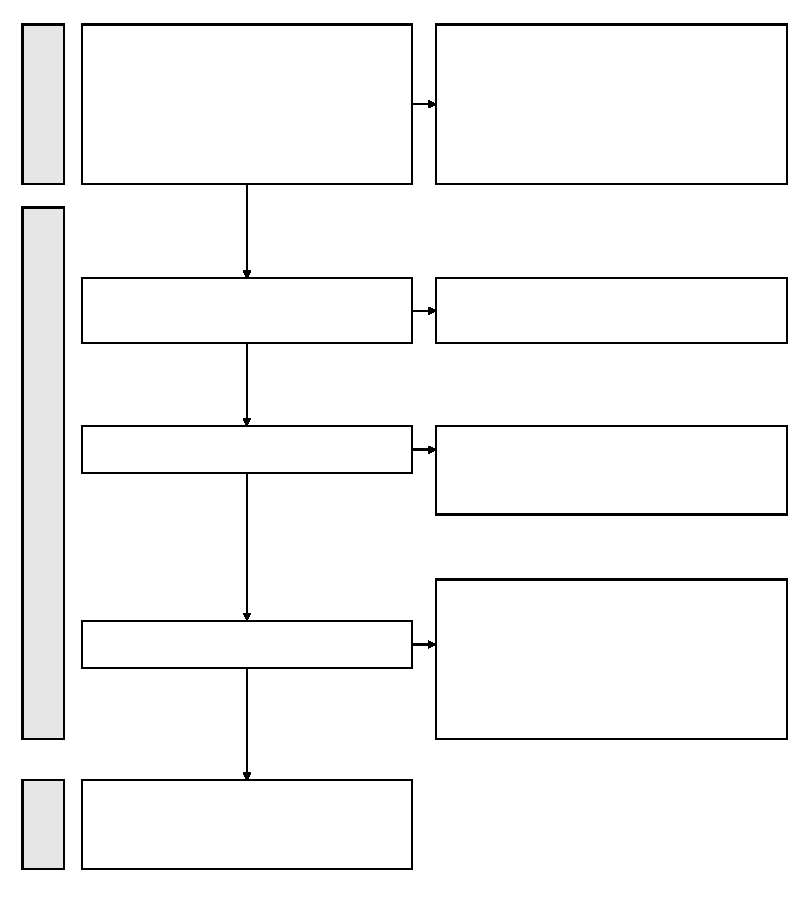
\includegraphics{Fig1}
\caption{PRISMA 2020 flow diagram for this review, which searched databases only; citation searching was not carried out. The left-hand boxes give the number of records or reports at each stage, from identification through screening to inclusion, and the right-hand boxes give the number removed or excluded at that stage, with the reasons}\label{fig:prisma}
\end{figure}

Of the 47 reports sought, 7 were not retrieved (Table~\ref{tab:notret}). Five were recorded as closed access at retrieval. For a sixth, Wang et al.'s AlertPro, only the publisher's landing page with the abstract and section snippets was obtained, which is not enough to assess the study. For the seventh, no full text is on file and no reason was recorded; this is an unresolved gap in the retrieval record. The remaining 40 reports were assessed for eligibility, and 6 were excluded (Table~\ref{tab:ftexcl}). Three described response actions but evaluated their models only as classifiers or detectors \citep{manojkumar2026,bompally2026,reddyavula2026}. One, the shielded incident-response agent of \citet{alauthman2026}, which the project's thematic review had treated as the closest precedent, reports an evaluation plan and ``indicative findings'' shown as arrows, but no measured values. One report was excluded as out of scope on manual judgement, and one because its full text is in French. In all, 34 studies, each described in one report, entered the synthesis: 20 from the first priority group and 14 from the second. Table~S1 of Online Resource~1 gives the outcome for every report sought.

\begin{table}[!htbp]
\caption{Reports sought for retrieval but not retrieved, with the identifier used in the screening record (ID), the report title and the reason it was not retrieved}\label{tab:notret}
\footnotesize
\begin{tabularx}{\textwidth}{@{}lLP{3.4cm}@{}}
\toprule
ID & Report & Reason \\
\midrule
S046 & Combating alert fatigue with AlertPro: Context-aware alert prioritization using reinforcement learning for multi-step attack detection & Closed access: only the publisher landing page (abstract and section snippets) was obtained \\
S058 & Digital Sovereignty by Design: Reinforcement Learning--Based Self-Healing for Cyber Resilience & Closed access (recorded at retrieval) \\
S068 & From Rules to Autonomy: Leveraging Reinforcement Learning for Real-Time Cyber Threat Mitigation & Closed access (recorded at retrieval) \\
S093 & Off-policy actor-critic deep reinforcement learning methods for alert prioritization in intrusion detection systems & Closed access (recorded at retrieval) \\
S108 & Reinforcement Learning with AI for Autonomous Incident Response in DevSecOps: Using RL Agents to Detect, Classify, and Mitigate Security Threats in Cloud-Native DevOps Environments & No full text on file and no reason recorded \\
S109 & Reinforcement Learning-Based Alert Prioritisation in Security Operation Centre: A Framework for Enhancing Cybersecurity in the Digital Economy & Closed access (recorded at retrieval) \\
S113 & Risk-Aware SOC Alert Handling in Adaptive Cyber Defense with Reinforcement Learning & Closed access (recorded at retrieval) \\
\botrule
\end{tabularx}
\end{table}

\begin{table}[!htbp]
\caption{Reports excluded at full-text assessment, with the identifier used in the screening record (ID), the report and the criterion and reason for its exclusion}\label{tab:ftexcl}
\footnotesize
\begin{tabularx}{\textwidth}{@{}lP{4.6cm}L@{}}
\toprule
ID & Report & Reason \\
\midrule
S016 & Adaptive NeuroDefense: Graph Neural Network and Reinforcement Learning-based Self-Healing Cybersecurity Architecture \citep{manojkumar2026} & EC3: evaluated only as a detector (accuracy on NSL-KDD, CICIDS-2017, UNSW-NB15); the DQN mitigation choices are not evaluated \\
S027 & AI-Powered Incident Response Framework for Secure DevOps Environments \citep{bompally2026} & EC3: the MDP action set is not specified and the agent is evaluated only with classification metrics (accuracy, AUC) \\
S065 & Explainable Reinforcement Learning for Automated Incident Response in Critical Infrastructure \citep{alauthman2026} & IC4: no quantitative evaluation. The paper specifies an evaluation plan and reports ``indicative findings'' as arrows, with no measured values \\
S072 & Hybrid LSTM-QEQ Framework for Enhanced Cyber Threat Detection and Response in Critical Power Grid Infrastructure & Out of scope (manual full-text judgement) \\
S104 & Reinforced Autonomous Agents with Attack-Defense Exercises in Realistic Environments & IC5: full text is not in English (French) \\
S130 & XAI for Automated Prediction Model for Cyber Incident Response and Security Support in Cloud \citep{reddyavula2026} & EC3: response actions are described, but the model is evaluated only as a classifier of 26 memory dumps (accuracy, AUC) \\
\botrule
\end{tabularx}
\end{table}

\subsection{Study Characteristics}

Table~\ref{tab:summary} summarises the 34 included studies, and Table~S2 of Online Resource~1 describes each one. The work is recent: 27 of the 34 studies were published in 2025 or 2026, 17 of them in 2026, and the earliest in 2020. Most of the evidence comes from security settings. Only 10 studies concern IT service and cloud operations, and all but one of these address root cause analysis or the remediation of faults in microservice and cloud systems; the exception prioritises incident reports \citep{peralta2025}. The other 24 studies concern alert triage in security operations centres (SOCs), incident response on enterprise and military networks, industrial and Internet of Things (IoT) systems, or digital forensics during incident response.

The environments are mostly constructed. Of the 34 studies, 13 built their own simulator and 6 used a public benchmark, chiefly the CAGE-2 and CAGE-4 cyber-defence gyms (Cyber Autonomy Gym for Experimentation) and the RCAEval root-cause benchmark; 6 replayed public datasets, most often intrusion-detection flow records regrouped into decision episodes, and 5 used emulated testbeds. Only 3 studies used operational data from an organisation \citep{peralta2025,wang2023hrlhf,ding2023}, and one evaluated on a physical testbed as well as a benchmark \citep{hammar2026belief}.

\begin{table}[!htbp]
\caption{Characteristics of the 34 included studies: the number of studies by setting, publication year, formulation of the decision problem and evaluation environment}\label{tab:summary}
\footnotesize
\begin{tabularx}{\textwidth}{@{}lLr@{}}
\toprule
Group & Category & Studies \\
\midrule
Setting & IT service and cloud operations & 10 \\
 & Security operations and alert triage & 6 \\
 & Network and enterprise incident response & 11 \\
 & Industrial, cyber-physical and IoT systems & 5 \\
 & Digital forensics during incident response & 2 \\
\midrule
Year & 2020 & 1 \\
 & 2022 & 2 \\
 & 2023 & 2 \\
 & 2024 & 2 \\
 & 2025 & 10 \\
 & 2026 & 17 \\
\midrule
Formulation\textsuperscript{a} & Explicit belief (POMDP) & 4 \\
 & Other partially observable formulation & 5 \\
 & Constrained MDP & 2 \\
 & Offline MDP & 1 \\
 & Game & 2 \\
 & Hierarchical & 3 \\
\midrule
Environment & Benchmark & 6 \\
 & Custom simulator & 13 \\
 & Emulated testbed & 5 \\
 & Testbed and benchmark & 1 \\
 & Public dataset & 6 \\
 & Operational data & 3 \\
\botrule
\end{tabularx}
\footnotetext{\textsuperscript{a}Formulation categories overlap; a study is counted in each that applies, and studies formulated as a fully observed MDP are not listed.}
\end{table}

\subsection{Quality of the Included Studies}

The quality of the evidence is uneven (Table~\ref{tab:qualsummary}). Of the 34 studies, 9 meet at least six of the eight checklist items, and 12 meet at most two. \citet{hammar2026belief} and \citet{sahin2026} meet all eight; \citet{nyberg2024} meet seven; \citet{peralta2025}, \citet{okafor2026}, \citet{rojasrodriguez2026}, \citet{ghanem2026}, \citet{hammar2025} and \citet{kovtun2026} meet six. The weakly rated studies typically report a single run without variance, do not test the agent on unseen conditions, and describe their environment or hyperparameters too briefly for the work to be repeated. Table~S4 of Online Resource~1 gives every rating.

Three weaknesses run across the set. Only 11 studies report results over several runs with a measure of variance, only 9 test their agents on conditions not seen in training, and only 5 give enough detail, with public code or environment, for the work to be repeated. A non-learning baseline is more common, met by 19. The synthesis below therefore gives most weight to the strongly rated studies and treats results from the weakest as indications only.

\begin{table}[!htbp]
\caption{Quality appraisal of the 34 included studies: for each checklist item (Q1--Q8; Table~\ref{tab:checklist}) the number of studies rated met, partly met (Part) or not met (Not)}\label{tab:qualsummary}
\footnotesize
\begin{tabularx}{\textwidth}{@{}lLrrr@{}}
\toprule
Item & Question & Met & Part & Not \\
\midrule
Q1 & Formulation & 25 & 9 & 0 \\
Q2 & Environment & 19 & 14 & 1 \\
Q3 & Non-learning baseline & 19 & 8 & 7 \\
Q4 & Metrics defined & 21 & 10 & 3 \\
Q5 & Repeated runs with variance & 11 & 7 & 16 \\
Q6 & Unseen test conditions & 9 & 10 & 15 \\
Q7 & Limitations & 19 & 7 & 8 \\
Q8 & Reproducible details & 5 & 17 & 12 \\
\botrule
\end{tabularx}
\end{table}

\subsection{Coverage of the Review Questions}

Table~\ref{tab:coverage} counts the studies that contain each element of the review questions, and Fig.~\ref{fig:coverage} shows the same counts against the size of the evidence base. Table~S3 of Online Resource~1 records the elements study by study. The counts are descriptive; no effect sizes were pooled, for the reasons given in Section~\ref{sec:method}.

\begin{table}[!htbp]
\caption{Number of included studies (of 34) that contain each element of the review questions, grouped into decisions, constraints, measures and evaluation}\label{tab:coverage}
\footnotesize
\begin{tabularx}{\textwidth}{@{}lLr@{}}
\toprule
Group & Element & Studies \\
\midrule
Decision & Gathers information (explicit action) & 17 \\
 & Takes or recommends a response or remediation action & 22 \\
 & Disposes of the alert (close, allow, prioritise) & 5 \\
 & Escalates, defers or hands off to a person & 7 \\
 & Information gathering and response action & 7 \\
 & Information gathering, response action and escalation & 1 \\
\midrule
Constraint & Hard filter or shield & 5 \\
 & Action masking & 6 \\
 & Expected-cost or budget constraint & 4 \\
 & Reward penalty only & 11 \\
 & None stated & 8 \\
 & Handling of a blocked action reported & 3 \\
\midrule
Measures & Decision quality & 31 \\
 & Investigation or time efficiency & 19 \\
 & Escalation behaviour & 5 \\
 & Constraint compliance & 4 \\
 & Three or more of the four groups & 5 \\
 & All four groups & 1 \\
\midrule
Evaluation & Non-learning (static or rule) baseline & 20 \\
 & Robustness tested & 15 \\
\botrule
\end{tabularx}
\end{table}

\begin{figure}[!htbp]
\centering
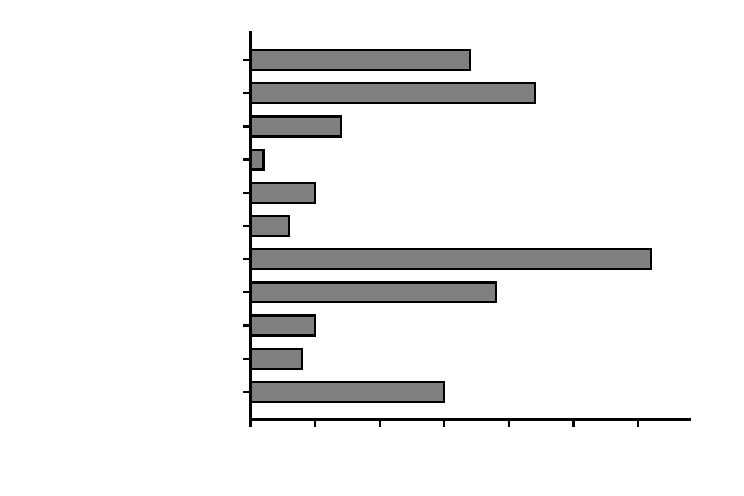
\includegraphics{Fig2}
\caption{Horizontal bar chart of the number of included studies, out of 34, that contain each element of the review questions. From top to bottom the bars show the decisions made (gathers information, response action, escalates or defers, all three decisions), constraint handling (hard filter or shield, blocked action handled), the measures reported (decision quality, efficiency, escalation, compliance) and robustness testing. Each bar is labelled with its count}\label{fig:coverage}
\end{figure}

\subsection{Synthesis for SRQ1: Formulation and Representation of Uncertain Evidence}

The answer to SRQ1 is that incident handling is formulated mostly as a fully observed MDP, and that explicit representation of uncertain evidence is the exception. Four themes support this answer.

\subsubsection{Explicit belief over a hidden incident state is used by a minority of studies}

Only 4 studies formulate the problem as a POMDP and act on a belief, a probability distribution over the hidden security state. \citet{hammar2026belief} estimate the belief with a particle filter and compute policies by belief aggregation and rollout; \citet{hammar2025} go further and hold a belief over the system model itself, updated by Bayesian learning as the incident unfolds. \citet{kovtun2026} track a belief over a hidden attack regime in a SOC, and \citet{koupaei2026} use a Dempster-Shafer belief for small-enterprise incident response. These are among the more strongly rated studies, so the representation the project needs exists and has been evaluated, although mainly on security benchmarks.

\subsubsection{Ambiguity is produced mainly by noisy, missing or overlapping evidence in a simulator, and it is usually fixed at one level}

\citet{koupaei2026} set false-positive and false-negative rates of 12\% and 18\%. \citet{contractor2025} lower the detection rate from 95\% to 50\% and add benign users who raise false alerts. \citet{sahin2026} design evidence that is stochastic and overlaps across classes, so that gathering evidence can lower confidence in a true threat or raise it for a benign alert, and add a hardened regime in which threats start at low confidence. \citet{wu2026} vary fault severity and change the link topology during episodes, \citet{peralta2025} model the vagueness of incident descriptions with fuzzy sets, and multi-agent studies give each agent only local observations \citep{aenugu2026,ravi2025}. Only a few of these studies treat the level of ambiguity as an experimental factor that is varied \citep{contractor2025,sahin2026,wu2026}.

\subsubsection{Many studies treat the incident state as a fully observed feature vector}

In about half the studies the state is a vector of metrics, alert scores or dataset features with no model of what the agent cannot see \citep{saeed2025,noorulhassan2026,alturkistani2022,bhosale2026,raj2026,nimmathi2026,yuan2026,babar2026,hughes2022,jaber2025,singh2026,ghanem2026,dunsin2025,wang2024mrca,ding2023}. In these studies ambiguity is assumed away rather than modelled, and the agent's decision cannot depend on how certain it is.

\subsubsection{No shared environment exists for IT service incident triage}

The security studies share benchmarks: CAGE-2 is used by three studies \citep{hammar2026belief,hammar2025,nyberg2024} and CAGE-4 or CybORG by two \citep{castro2025,contractor2025}, and RCAEval serves root cause analysis \citep{rojasrodriguez2026}. Three studies repurpose intrusion-detection datasets as alert streams or decision episodes \citep{okafor2026,kovtun2026,alturkistani2022}. Apart from the root-cause studies that use RCAEval or open microservice benchmarks, the IT service studies each build their own fault-injection setup or use one organisation's data \citep{peralta2025,wang2023hrlhf,ding2023,wu2026,yuan2026}. Results from different IT service studies therefore cannot be compared directly.

\subsection{Synthesis for SRQ2: The Decisions the Agents Make}

The answer to SRQ2 is that gathering information and acting are common decisions, escalation to a person is rare, and no study learns one policy over all three for IT service incidents. Four themes support this answer.

\subsubsection{Information gathering is an explicit, costed action in half the studies}

A total of 17 studies give the agent an action whose purpose is to obtain evidence. In security settings it takes the form of an analyse or investigate action \citep{hammar2026belief,hammar2025,nyberg2024,castro2025,contractor2025,okafor2026}, queries to logs and threat intelligence \citep{sahin2026}, a choice of which alerts analysts should investigate within a budget \citep{tong2020}, a decision to defer and gather context \citep{kovtun2026}, increased logging \citep{jaber2025}, or the next step of a forensic examination \citep{ghanem2026,dunsin2025}. In root cause analysis it is the choice of which part of the system to examine next, whether to stop, or which components to exclude \citep{rojasrodriguez2026,wang2024mrca,wu2026,ding2023}, and \citet{wang2023hrlhf} let the agent choose which dependencies to ask engineers about.

\subsubsection{Where investigation is available, it reduces errors or effort}

\citet{wu2026} report 3.2 investigation steps on average against 6.1 for a plain deep Q-network (DQN), with higher accuracy. \citet{kovtun2026} find that the option to defer cut false escalations from 7.2\% to 5.0\% and from 9.4\% to 6.6\% on two datasets. \citet{ghanem2026} report investigation time cut by up to 68\% against analyst-assisted baselines, and \citet{wang2023hrlhf} reduce the number of questions put to engineers from $\mathrm{O}(N^{2})$ to $\mathrm{O}(1)$. These results support treating investigation as a decision with a cost, as the project does.

\subsubsection{Escalation to a person is rarely a learned action}

Only 7 studies include escalation, deferral or hand-off to a person. \citet{bhosale2026} let a DQN choose to allow, monitor or escalate phishing alerts, where escalation opens a ServiceNow incident, and \citet{alturkistani2022} train a DQN to fix an alert or escalate it to the next tier of SOC operators. \citeauthor{sahin2026}'s \citeyearpar{sahin2026} agent can escalate to incident response, and a separate layer defers the most uncertain alerts to an analyst; \citeauthor{kovtun2026}'s \citeyearpar{kovtun2026} agent escalates to deep analysis. In the other three the hand-off is fixed by design rather than learned: \citet{okafor2026} leaves containment to analysts in the deployed system, \citet{singh2026} routes an action to a human when a deterministic safety check fails, and \citet{koupaei2026} include notifying a managed security provider as a playbook. Six of the 7 are in security operations or incident response. The only IT service study among them, Singh's, hands off when a rule check fails; none of the 10 IT service studies learns when to escalate.

\subsubsection{No study learns one policy over investigating, remediating and escalating for IT service incidents}

Only 1 study combines an information-gathering action, a response action and escalation: \citeauthor{okafor2026}'s \citeyearpar{okafor2026} offline agents choose to dismiss, investigate or contain SOC alerts, and analyst ownership of containment is a deployment decision, not a learned one. \citet{sahin2026} combine evidence gathering with escalation and closure but have no remediation action, and \citet{kovtun2026} combine shallow triage, deep analysis and deferral, again without remediation. The three-way decision the project studies is therefore not covered in the evidence base; the nearest work is security alert triage.

\subsection{Synthesis for SRQ3: Enforcement of Operational Constraints}

The answer to SRQ3 is that constraints are most often encoded as reward penalties, that hard rule enforcement is proposed more often than it is measured, and that what replaces a blocked action is almost never reported. Reward penalties are the most common mechanism. A total of 11 studies express their operational limits only as penalties in the reward: for destructive self-healing actions \citep{yuan2026}, for restoring hosts \citep{nyberg2024,hammar2026belief,hammar2025}, for under-escalation \citep{bhosale2026}, or for violating an organisation's response policy encoded as a reward profile \citep{hughes2022}. A further 8 state no constraint at all. A penalty discourages a prohibited action but does not prevent it, which is the distinction the project's design depends on \citep{konighofer2025}. Four themes describe the studies that go further.

\subsubsection{Action masking and expected-cost constraints are the common lightweight alternatives}

In 6 studies, actions that are invalid or unsafe in the current state are masked. \citet{contractor2025} unmask the disruptive restore action only when a persistent threat is present, and the analyse action only after a detection or a message from another agent; root-cause and forensic studies mask expanded nodes or restrict actions to a pool derived from engineers \citep{wang2024mrca,rojasrodriguez2026,ding2023,ghanem2026,wu2026}. Another 4 bound an expected cost or a budget. \citet{kovtun2026} constrain both the use of deep analysis and the attack-miss rate, and report that both constraints held in 14 of 15 seeds on one dataset and 13 of 15 on the other; \citet{sahin2026} certify error budgets on benign escalation and on threats closed automatically, realising rates of 0.0099 and 0.0101 against budgets of 0.01.

\subsubsection{Hard runtime filters are proposed, but only two studies measure them}

In 5 studies, proposals are checked against rules at run time. \citet{ravi2025} check every proposed action against legal, service-level and safety rules and replace a violating action with a safer alternative or a no-op, with a penalty. \citet{singh2026} restricts the agent to a feasible action region and adds a deterministic execution guard. \citet{koupaei2026} restrict the allowable action set by cost and time limits, \citet{elicha2026} let expert rules handle known threats before the RL agent sees an alert, and \citet{okafor2026} adds a severity floor that prevents medium- and high-severity alerts from being dismissed automatically. Only Ravi et al.\ and Singh report how the rules behaved: \citeauthor{ravi2025}'s \citeyearpar{ravi2025} shield intervened 526 to 623 times per scenario, and removing \citeauthor{singh2026}'s \citeyearpar{singh2026} guard left the mean time to resolution almost unchanged (142\,s to 144\,s) but cut the governance compliance rate from 99.9\% to 72.3\%.

\subsubsection{What happens to a blocked decision is reported in 3 studies}

\citet{ravi2025} substitute an alternative or a no-op, \citet{singh2026} hands the action to a human, and \citet{sahin2026} defer to an analyst any alert that cannot be decided within the error budgets. None of the studies lets the agent propose again after a block, which is the project's rule.

\subsubsection{Rule enforcement changes behaviour and has a cost}

\citeauthor{singh2026}'s \citeyearpar{singh2026} guard bought compliance at almost no cost in resolution time. In \citeauthor{ravi2025}'s \citeyearpar{ravi2025} study the cost was larger: the shielded agent took 9 to 11 times more false actions and incurred 74--77\% higher cost than an unshielded proximal policy optimisation (PPO) agent, while detecting far more attacks (recall 0.96--0.99 against 0--0.084). This study is weakly rated, and its text reports that the PPO agent proposed unsafe actions although that agent ran without a shield, so its comparison should be read with caution.

\subsection{Synthesis for SRQ4: Environments, Baselines and Metrics}

The answer to SRQ4 is that the studies measure the quality of the final decision and the time taken, but rarely escalation behaviour or compliance, and that their reporting is often too weak for the results to be compared. Three themes support this answer.

\subsubsection{Decision quality and time dominate; escalation and compliance are rarely measured}

Decision quality is measured in 31 studies, through accuracy, reward, cost, recall or the Matthews correlation coefficient (MCC), and 19 studies measure time or investigation effort, most often as mean time to recovery \citep{singh2026,koupaei2026,nimmathi2026,aenugu2026}. Only 5 measure escalation behaviour \citep{peralta2025,sahin2026,nimmathi2026,bhosale2026,kovtun2026} and 4 constraint compliance \citep{singh2026,sahin2026,kovtun2026,ravi2025}. One study, \citet{kovtun2026}, reports measures in all four groups, for SOC alert escalation. \citet{peralta2025} report the clearest operational effect on escalation: in a deployment trial, the escalation rate fell from 11.8\% to 9.2\% and manual priority overrides from 15.2\% to 6.2\%, although this was a before--after comparison without a control.

\subsubsection{A static or rule-based comparison is common but not universal}

In all, 20 studies compare against a non-learning policy: static thresholds, fixed scripts, playbooks, heuristics, a periodic recovery policy, or human examiners \citep{hammar2026belief,koupaei2026,bhosale2026,wu2026,yuan2026,aenugu2026,ghanem2026}. The others compare only learning methods with each other, compare with values reported by other studies, or have no baseline \citep{saeed2025,noorulhassan2026,khozam2025,elicha2026,hughes2022,jaber2025,alturkistani2022}. The extracted results contain no case in which a static baseline outperformed the learned policy on a study's main measure. How much this reflects the strength of the learned policies and how much the weakness of the baselines cannot be separated from the reports.

\subsubsection{Reporting weaknesses limit the comparisons}

Several studies show how the choice of metric can mislead. \citet{okafor2026} found that value-based offline RL and a Decision Transformer degenerated into trivial detectors whose failure the F1 score and the area under the receiver operating characteristic curve (ROC-AUC) concealed and MCC revealed. \citeauthor{ravi2025}'s \citeyearpar{ravi2025} PPO baseline scored 0.98 accuracy with near-zero recall. \citet{sahin2026} report that an earlier version of their simulator leaked the label into the confidence signal, so that any threshold appeared to achieve perfect recall, and recommend checks against this defect. Several weaker studies contain internal inconsistencies: two different improvement figures for the same result \citep{koupaei2026,varsha2025}, a train--test split that is stated but not used \citep{bhosale2026}, an action in a worked example that is absent from the action set \citep{jaber2025}, and training and testing on the same stream \citep{alturkistani2022}.

\subsection{Synthesis for SRQ5: Robustness to Ambiguity and Change}

The answer to SRQ5 is that robustness is tested in under half the studies, mostly for the quality of the final decision, and that no study measures how the mix of investigating, acting and escalating changes as evidence becomes more ambiguous. Three themes support this answer.

\subsubsection{Robustness is tested through model error, change, unseen attackers and weaker detection}

A total of 15 studies test their agents under conditions that differ from training: a misspecified model of the system \citep{hammar2025}, a non-stationary system \citep{hammar2026belief}, unseen attacker profiles and network structures \citep{ravi2025,nyberg2024,castro2025}, a lower detection rate \citep{contractor2025}, dataset shift \citep{sahin2026}, terminology drift \citep{peralta2025}, dynamic topology \citep{wu2026}, and load near capacity \citep{aenugu2026,kovtun2026}. Performance generally degrades but does not collapse: \citeauthor{peralta2025}'s \citeyearpar{peralta2025} accuracy fell from 82.9\% to 79.4\% under drift, \citeauthor{aenugu2026}'s \citeyearpar{aenugu2026} mean time to recovery rose from 41.2\,s to 79.4\,s at peak load, and \citeauthor{nyberg2024}'s \citeyearpar{nyberg2024} graph agents worked on unseen networks without retraining but scored below agents trained on each network.

\subsubsection{Methods that maintain a belief or adapt their model degrade least}

Under a misspecified model, \citeauthor{hammar2025}'s \citeyearpar{hammar2025} method incurred a cost of 35.91 against 91.51 or more for every other method, although it was slightly worse than the best methods when the model was correct. \citeauthor{hammar2026belief}'s \citeyearpar{hammar2026belief} method adapted its policy to a system change in about 15\,s to 19\,s, against more than 30\,min for PPO, and PPO's results varied about ten times more. Both studies are strongly rated.

\subsubsection{As ambiguity rises, deferral to people rises; how the full decision mix shifts is unmeasured}

\citet{sahin2026} show that when the scoring model degrades under dataset shift, the share of alerts deferred to analysts rises, to 79--99\% for the most affected classifiers, so that failure becomes visible instead of silent. \citet{kovtun2026} show that deferring to gather context reduces false escalations, and \citet{contractor2025} show that lower detection rates lower returns and that unmasking investigation on a message from another agent recovers part of the loss. No study reports the shares of investigating, acting and escalating at increasing levels of ambiguity.

\subsection{Thematic Traceability}\label{sec:trace}

Table~\ref{tab:trace} links each review question to its themes, the studies that support each theme, and the interpretation drawn. It is the basis of the discussion that follows.

{\scriptsize
\begin{longtable}{@{}lP{2.7cm}P{4.3cm}P{3.7cm}@{}}
\caption{Thematic traceability matrix: for each review question (SRQ), the themes identified, the studies that support each theme and the interpretation drawn. Study identifiers such as S038 are those of the decision log (Table~S1 in Online Resource~1)}\label{tab:trace}\\
\toprule
SRQ & Theme & Supporting studies & Interpretation \\
\midrule
\endfirsthead
\caption[]{(continued)}\\
\toprule
SRQ & Theme & Supporting studies & Interpretation \\
\midrule
\endhead
\botrule
\endfoot
SRQ1 & Explicit belief over a hidden incident state is used by a minority of studies & \citealp{hammar2026belief,hammar2025,koupaei2026,kovtun2026} & The representation the project needs exists and has been evaluated, mostly on security benchmarks \\
 & Ambiguity is produced mainly by noisy, missing or overlapping alerts in simulators & \citealp{koupaei2026,contractor2025,sahin2026,wu2026,peralta2025,aenugu2026,ravi2025} & Few studies vary ambiguity as an experimental factor; most fix it at one level \\
 & Many studies treat the incident state as a fully observed feature vector & \citealp{saeed2025,noorulhassan2026,alturkistani2022,bhosale2026,raj2026,nimmathi2026,yuan2026,babar2026,hughes2022,jaber2025,singh2026,ghanem2026,dunsin2025,wang2024mrca,ding2023} & Ambiguity is often assumed away rather than modelled \\
 & Evaluation environments are mostly security benchmarks, custom simulators and repurposed intrusion detection system (IDS) datasets & \citealp{hammar2026belief,hammar2025,castro2025,contractor2025,nyberg2024,rojasrodriguez2026,okafor2026,kovtun2026,sahin2026,peralta2025,wang2023hrlhf,ding2023} & No shared environment exists for IT service incident triage \\
\midrule
SRQ2 & Information gathering is an explicit action in about half the studies & \citealp{okafor2026,hammar2026belief,rojasrodriguez2026,sahin2026,tong2020,castro2025,contractor2025,ghanem2026,jaber2025,wang2024mrca,hammar2025,dunsin2025,wu2026,kovtun2026,wang2023hrlhf,nyberg2024,ding2023} & Investigation is treated as a decision with a cost, as the project assumes \\
 & Escalation to a human is rarely a learned action & \citealp{bhosale2026,alturkistani2022,sahin2026,kovtun2026,okafor2026,singh2026,koupaei2026} & Where escalation exists it is mostly in security alert triage, and S038 hands off by rule rather than by learning \\
 & No study learns one policy over investigating, remediating and escalating for IT service incidents & \citealp{sahin2026,okafor2026,kovtun2026} & The three-way decision of the project is not covered; the nearest work is security alert triage \\
 & When investigation is available it reduces errors or effort & \citealp{wu2026,kovtun2026,ghanem2026,wang2023hrlhf} & Supports giving the agent a costly investigate action \\
\midrule
SRQ3 & Hard runtime filters and shields are proposed but rarely measured & \citealp{ravi2025,singh2026,koupaei2026,elicha2026,okafor2026} & Only S118 and S038 report how often rules intervened or were complied with \\
 & Action masking and expected-cost constraints are the common lightweight alternatives & \citealp{contractor2025,rojasrodriguez2026,wang2024mrca,ghanem2026,wu2026,ding2023,kovtun2026,tong2020,varsha2025,sahin2026} & Masking prevents prohibited proposals rather than reacting to them \\
 & What happens to a blocked action is reported in only three studies & \citealp{ravi2025,singh2026,sahin2026} & The project's rule of one re-proposal then escalation has no direct precedent \\
 & Rule enforcement changes behaviour and has a cost & \citealp{singh2026,ravi2025} & Compliance has to be measured alongside decision quality and cost \\
\midrule
SRQ4 & Decision quality and time dominate the metrics; escalation and compliance are rarely measured & All 34 (Table~S4 in Online Resource~1) & Only one study measures all four groups the project plans, and it concerns SOC alert escalation \\
 & A static or rule-based comparison is common but not universal & \citealp{peralta2025,hammar2026belief,singh2026,babar2026,rojasrodriguez2026,koupaei2026,sahin2026,tong2020,nimmathi2026,castro2025,ghanem2026,varsha2025,wang2024mrca,aenugu2026,bhosale2026,dunsin2025,wu2026,wang2023hrlhf,yuan2026,ding2023} & A rule-based baseline is standard and the project should keep one \\
 & Reporting weaknesses limit the comparisons & \citealp{okafor2026,ravi2025,koupaei2026,bhosale2026,varsha2025,jaber2025,alturkistani2022,sahin2026} & Metrics such as MCC, per-class recall and seed variance are needed \\
\midrule
SRQ5 & Robustness is tested through model error, change, unseen attackers and weaker detection & \citealp{hammar2025,hammar2026belief,ravi2025,nyberg2024,contractor2025,sahin2026,peralta2025,wu2026,aenugu2026,castro2025,kovtun2026} & Robustness is tested in about a third of studies, mostly for decision quality \\
 & Methods that maintain a belief or adapt their model degrade least & \citealp{hammar2025,hammar2026belief} & Supports explicit belief tracking in the project agent \\
 & As ambiguity rises, deferral to people rises; how the full decision mix shifts is unmeasured & \citealp{sahin2026,kovtun2026,contractor2025} & No study reports the shares of investigating, acting and escalating across ambiguity levels \\
\end{longtable}
}

\section{Discussion}
\label{sec:discussion}

This review set out to find how RL has been applied to IT incident handling, which decisions the agents make, how rules are enforced, and how the agents are evaluated. The 34 included studies show that each part of the planned design has been studied somewhere, but not together and seldom for IT service incidents. This section interprets the findings for each review question, returns to the gaps stated in Table~\ref{tab:objectives}, and sets out what the findings imply for the project.

\subsection{Representation of Uncertain Evidence}

The thematic review stated that the environments in the literature model cyberattacks and microservice faults and that none lets the ambiguity of IT service incidents be varied. The systematic search confirms this gap and sharpens it. Belief-based formulations exist and perform well under change \citep{hammar2026belief,hammar2025}, but all 4 studies that use them concern security incidents. The IT service studies are almost all root cause analysis on microservice benchmarks or on one company's data, and they treat the system's metrics as fully observed. Three studies vary the level of ambiguity as an experimental factor \citep{contractor2025,sahin2026,wu2026}; none of them concerns user-reported IT service incidents.

There are two ways to read this. One is that IT service triage does not need a model of hidden state because its evidence is good enough. The studies give no support for this reading, since none tests it. The other is that the field has not yet built an environment in which the question can be asked. \citeauthor{chen2020}'s \citeyearpar{chen2020} observation that distinct problems produce similar symptoms favours the second reading. A simulator in which the overlap between incident causes can be set, as \citet{sahin2026} do for alert classes, would let the question be tested directly.

\subsection{The Three Decisions}

The thematic review found that information gathering and deferral had been studied separately. The included studies agree. Investigation is an explicit action in 17 studies, and where it is measured it reduces either errors or effort \citep{wu2026,kovtun2026,ghanem2026,wang2023hrlhf}. Escalation is much rarer, and where it is present it is often fixed by design: a severity floor, a rule-triggered hand-off, or a playbook \citep{okafor2026,singh2026,koupaei2026}. Only one study combines all three kinds of decision, and its escalation is not learned \citep{okafor2026}.

The closest work to the project is therefore in security alert triage, not IT service management. \citeauthor{sahin2026}'s \citeyearpar{sahin2026} system gathers evidence, escalates or closes, and defers the uncertain cases to an analyst under certified error budgets. \citeauthor{kovtun2026}'s \citeyearpar{kovtun2026} agent chooses between shallow triage, deep analysis and deferral under a cost constraint. Both are strongly rated, and both treat escalation as a decision with a cost, as \citet{turan2026} argues it should be. Neither recommends a remediation. The project's question is whether one policy can learn to make the choice between all three when the third option is a fix with operational consequences. The evidence does not answer that question; it shows the parts that have worked separately.

\subsection{Enforcement of Operational Rules}

The thematic review found that shields had been demonstrated mainly on control tasks \citep{alshiekh2018,konighofer2025}, and that the one shielded incident-response agent it identified had not reported how its mechanism behaved \citep{alauthman2026}. The systematic search confirms that study's status: it reports an evaluation plan and indicative findings, not measurements, and it was excluded on that ground. The 5 included studies with a hard filter show that the idea has reached incident handling, but only two report what the filter did \citep{ravi2025,singh2026}.

Those two results point in different directions. \citeauthor{singh2026}'s \citeyearpar{singh2026} guard raised governance compliance from 72.3\% to 99.9\% at almost no cost in resolution time. \citeauthor{ravi2025}'s \citeyearpar{ravi2025} shield intervened hundreds of times per scenario and the shielded agent took many more false actions than an unshielded one. The difference may lie in how often the agent proposes prohibited actions, which depends on how it was trained. If the agent learns with the shield in place, as \citet{alshiekh2018} propose, it can learn to avoid proposals that will be blocked. Neither study reports the rate of blocked proposals over training, so this explanation cannot be checked from the evidence.

The more important finding for the project is what is missing. Only 3 studies say what happens after a block, and none lets the agent propose again. The project's rule, that a blocked agent may make one further proposal before the incident is escalated, has no direct precedent. Its effect on escalation rates and on the time to resolution will have to be measured, not assumed.

\subsection{Environments, Baselines and Metrics}

The thematic review stated that decision quality, investigation cost, escalation and constraint compliance had each been measured but not together. The systematic search finds one exception, \citet{kovtun2026}, who measure all four for SOC alert escalation. The rest measure decision quality and time, and few measure escalation or compliance. For an agent whose purpose is to choose between investigating, acting and escalating, decision quality alone is not enough: an agent that escalates every incident makes no wrong fix, and an agent that never escalates may look efficient. Measures of escalation and compliance are needed to see either failure.

The quality appraisal adds a caution about baselines and reporting. A non-learning baseline is common, and the learned policy always beat it in the extracted results, but few studies report variance across runs or test on unseen conditions. Okafor's and Ravi et al.'s results show how a single metric can hide a degenerate policy \citep{okafor2026,ravi2025}, and \citeauthor{sahin2026}'s \citeyearpar{sahin2026} account of label leakage in their own simulator shows how a simulator can make a policy look better than it is. These are the failure modes the project's evaluation is most exposed to, because it too will train and test in a simulator it builds.

\subsection{Robustness}

The thematic review found that robustness had been tested for decision accuracy and for the validity of shields, but not for the mix of investigating, recommending and escalating. The systematic search confirms this. In 15 studies the agents are tested under changed conditions, and the methods that maintain a belief or adapt their model degrade least \citep{hammar2025,hammar2026belief}. \citet{sahin2026} show the most relevant pattern: as the scoring model degrades, more alerts are deferred to people, so that failure becomes visible. No study reports how the shares of the three decisions change as evidence becomes more ambiguous. That curve is what the project's fifth research question asks for.

\subsection{Relevant Excluded Studies}

Two groups of excluded reports bear on the interpretation. The first is the shielded incident-response agent of \citet{alauthman2026}, which the thematic review treated as the closest precedent. Its exclusion leaves no included study that combines a shield with incident response in IT operations and reports measurements. The second is three reports that describe response actions but evaluate their models as classifiers \citep{manojkumar2026,bompally2026,reddyavula2026}. They show a common pattern in the wider literature: a framework is described as autonomous response, but what is evaluated is detection. A reader who counts such papers as evidence of RL-based response would overestimate how much of that evidence exists.

\subsection{Implications for the Project}

Fig.~\ref{fig:evidence} places the project against the evidence. Each of its four components has a precedent among the included studies, mostly in security settings, and the combination has none. The findings suggest six things for the project's design and evaluation.

\begin{enumerate}
\item The simulator should let the level of ambiguity be set, by controlling how far the symptoms of different causes overlap and how reliable each diagnostic check is, so that robustness can be measured as a function of it \citep{sahin2026,contractor2025}.
\item The agent should be compared with a learning baseline that keeps a belief, not only with a fully observed one, because belief-based methods were the most robust in the included studies \citep{hammar2025,hammar2026belief}.
\item Escalation should be a learned action with a cost, and its rate should be reported alongside decision quality, so that an agent which escalates everything cannot appear safe \citep{kovtun2026,turan2026}.
\item The rule mechanism should log every block, the re-proposal that follows, and whether the incident was then escalated, because no included study reports this sequence.
\item Results should be reported over several seeds with variance, with more than one decision-quality metric, and with checks for label leakage in the simulator \citep{okafor2026,sahin2026}.
\item The static, rule-based baseline should be as strong as a competent support team would use, because a weak baseline makes any learned policy look good.
\end{enumerate}

\begin{figure}[!htbp]
\centering
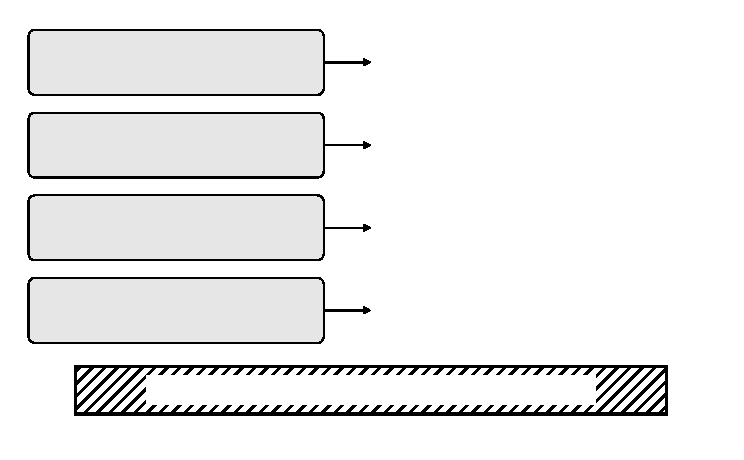
\includegraphics{Fig3}
\caption{Components of the planned agent (left column) and the included evidence for each (right column). Explicit belief over the hidden incident cause: 4 studies, all in security \citep{hammar2026belief,hammar2025,kovtun2026,koupaei2026}. Costed investigate action: 17 studies, with effort reduced in \citep{wu2026,kovtun2026}. Learned escalation: 7 studies, learned in four, all in security \citep{bhosale2026,alturkistani2022,sahin2026,kovtun2026}. Rule mechanism with blocked-action handling: 5 studies with hard filters, of which 3 report how a blocked action is handled and none allows a re-proposal. The hatched box at the bottom states that no study combines all four components for IT service incidents}\label{fig:evidence}
\end{figure}

\section{Limitations}
\label{sec:limitations}

The limitations of this review lie in the evidence it found and in the way it was conducted.

\subsection{Limitations of the Evidence}

Most of the evidence comes from simulation. Of the 34 studies, 13 built their own simulator, and only 3 used an organisation's operational data. Results from a simulator show what a policy can learn from the dynamics its authors chose, not how it will behave on real incidents. The evidence also leans towards security. Of the 34 studies, 24 concern security operations, incident response, industrial systems or forensics, and most of the 10 IT service studies concern root cause analysis rather than triage. Findings carried over from security alert triage to IT service incidents assume that the two decision problems are alike, which the studies do not test.

The quality of the evidence is uneven. Of the included studies, 12 meet at most two of the eight checklist items, only 11 report variance over repeated runs, and only 5 give enough detail to repeat the work. Several studies contain internal inconsistencies (Section~\ref{sec:results}). The checklist itself was written for this review and has not been validated, so the ratings indicate reporting quality and should not be read as a measure of risk of bias. The studies differ too much in task, environment and metric for their results to be pooled, so the synthesis is narrative and the counts are descriptive.

\subsection{Limitations of the Review Process}

The search may have missed relevant studies. Only three databases were searched, and Web of Science and arXiv were not among them. The IEEE Xplore search was limited to open-access records and returned 5, so IEEE studies behind a paywall that Scopus does not index are missing. The ACM Digital Library export reached its limit of 1000 records, so records beyond that limit were not seen; most of the exported ACM records were proceedings volumes, which suggests that the all-fields search was too broad for that library. The year terms in the Scopus and ACM strings do not restrict publication year, and the year filter was applied afterwards by the script. Citation searching was planned but not carried out, and at least one known relevant study was therefore not found \citep{ren2025}.

Automated filtering removed 4195 records by applying the string blocks to titles, abstracts and keywords. A relevant study that uses none of the method terms in these fields would have been removed without being read. Records without an abstract were judged on their titles alone.

Seven reports could not be assessed. Five were closed access, only the landing page of a sixth was obtained, and for the seventh no full text is on file and no reason was recorded. One report was excluded because its full text is in French. The review cannot say whether these eight reports would have changed its findings; at least three of the unretrieved reports concern SOC alert prioritisation, which is close to the review's focus.

Screening and extraction were not duplicated. The title and abstract decisions, the full-text assessments of the reports on file, the extraction and the quality ratings were made with an AI assistant, and two full-text decisions were made manually. The decision log, the extraction file and the quality ratings are provided so that every decision can be checked. Finally, the review was written to prepare for a particular study, and the themes were coded against that study's design. Section~\ref{sec:screening} and Table~S1 of Online Resource~1 state the decisions that required interpretation so that a reader can judge whether this framing affected them.

\section{Future Research}
\label{sec:future}

The gaps identified by this review suggest four directions for research, and two for the review itself.

The first is an environment for IT service incident triage in which the ambiguity of the evidence can be controlled. No such environment was found. It should let a researcher set how far the symptoms of different causes overlap and how reliable each diagnostic check is, and it should be released with its code so that results can be compared across studies, as the CAGE gyms allow for cyber defence.

The second is a single policy that learns to investigate, recommend a fix or escalate, evaluated against both a static policy and learning baselines with and without a belief. The security studies of \citet{sahin2026} and \citet{kovtun2026} show that parts of this design work for alerts; whether they work together when one option changes the system is an open question.

The third is the behaviour of rule enforcement when the agent can also investigate or escalate. Studies should report how often proposals are blocked during training and evaluation, what replaces a blocked proposal, and how blocking changes the rates of investigation and escalation. Only 3 included studies report any part of this.

The fourth is evaluation practice. Studies should report decision quality, investigation cost, escalation behaviour and compliance together; results over several seeds with variance; and performance as a function of ambiguity, including the shares of the three decisions at each level. Checks for label leakage in simulators, of the kind \citet{sahin2026} describe, should be routine.

For the review itself, the citation searching that was planned should be carried out, and the IEEE Xplore and ACM Digital Library searches should be repeated, the first without the open-access limit and the second restricted to titles, abstracts and keywords. The seven reports that could not be retrieved should be obtained and assessed.

\section{Conclusion}
\label{sec:conclusion}

This review searched three databases for studies that apply RL or sequential decision-making to IT incident handling, screened 131 records, and included 34 studies. Its findings answer the five review questions. Most studies formulate incident handling as a fully observed MDP, and only 4 keep an explicit belief over the hidden state. Information gathering is a common action, but escalation to a person is rare and often fixed by design, and only one study combines gathering, acting and escalating. Rule enforcement is usually a reward penalty; hard filters appear in 5 studies, and only 3 say what happens to a blocked decision. Decision quality is measured almost everywhere, while escalation and compliance are measured in few studies, and robustness is tested for the final decision but not for the mix of decisions.

The parts of an agent that investigates, acts or escalates under explicit rules have each been studied, mostly for security incidents, but no included study combines them for IT service incidents. The evidence is recent, largely simulated and uneven in quality. Within those limits, the review supports the project's plan to study such an agent, and it indicates what the evaluation must include: controlled ambiguity, learned escalation with a cost, a record of every blocked proposal, and measures of escalation and compliance reported alongside decision quality.

\backmatter

\bmhead{Supplementary information}
The online version contains supplementary material.
\textbf{Online Resource 1} (ESM\_1.pdf): Tables S1--S4, which give the outcome of every report sought for retrieval (S1), the task, formulation, environment and main result of each included study (S2), the coding of the review-question elements for each included study (S3), and the quality rating of each included study on items Q1--Q8 (S4).
\textbf{Online Resource 2} (ESM\_2.xlsx): the audit files of the review, one worksheet each: the decision and reason for each of the 131 screened records, the outcome for each of the 47 reports sought, the data extraction form and the quality ratings of the 34 included studies, the study and thematic traceability matrices, and the reconciliation of every PRISMA count.

\section*{Statements and Declarations}

\bmhead{Funding}
\tbc{Choose one: ``No funding was received for conducting this study.'' or ``This work was supported by [funder, written in full] (Grant number [...]).''}

\bmhead{Competing interests}
\tbc{To confirm: The author has no relevant financial or non-financial interests to disclose. The review was carried out to inform the author's own undergraduate research project on a reinforcement learning agent for IT incident triage (Section~\ref{sec:intro}).}

\bmhead{Ethics approval and consent to participate}
Not applicable. This review synthesises published studies; it involved no human participants, personal data or animals.

\bmhead{Consent for publication}
Not applicable.

\bmhead{Data availability}
The audit files that support the findings of this review are available in \tbc{repository name} \citep{opol2026data}: the decision and reason for every screened record (\texttt{exclusion\_traceability.csv}), the outcome of every report sought (\texttt{fulltext\_decisions.csv}), the extraction form (\texttt{data\_extraction.csv}), the quality ratings (\texttt{quality\_appraisal.csv}), the study and thematic traceability matrices, the reconciliation of every PRISMA count (\texttt{prisma\_reconciliation.csv}), and the screening and table-generation scripts. The same files are provided as Online Resource~2. The raw database exports and the full texts of the included studies are not shared, because the database licence terms and the publishers' copyright restrict their redistribution; the exports can be recreated by running the search strings in Table~\ref{tab:strings}.

\bmhead{Materials and code availability}
The scripts that combined the exports, applied the automated filters and generated the tables and counts are included in the repository cited under Data availability \citep{opol2026data}. No other materials were produced.

\bmhead{Author contributions}
Charis Opol is the sole author. She conceived and designed the review, ran the database searches, retrieved the full texts, conducted the screening, data extraction and quality appraisal with the AI assistance described in Section~\ref{sec:ai}, synthesised the evidence, and wrote and revised the manuscript. She read and approved the final manuscript.

\bmhead{Use of artificial intelligence tools}
The use of an AI assistant in conducting this review is described in Section~\ref{sec:ai}.

\bmhead{Prior dissemination and re-use of material}
This review was prepared during the author's undergraduate research project at Uganda Christian University. Parts of the Introduction (the description of incident management and triage, the framing of triage as a sequence of decisions, and the requirements for rule enforcement and escalation) and the gap statements in Table~\ref{tab:objectives} draw on, and in places repeat wording from, Chapters One and Two of the author's project report, \emph{Investigate, Recommend or Escalate: A Rule-Constrained Reinforcement Learning Agent for IT Incident Triage under Ambiguous Evidence} (Uganda Christian University, 2026), which also summarises some findings of this review. \tbc{To confirm: the report is an unpublished university assessment document and has not been published or submitted to any journal.}

\bibliography{references}

\end{document}
